
\documentclass[a4paper,14pt]{extreport}
\usepackage[utf8]{inputenc}
\usepackage[T2A]{fontenc}
\usepackage[russian]{babel}
\usepackage{amssymb,amsfonts,amsmath}
\usepackage{multicol}
\usepackage{graphicx}
\usepackage{listings}
\usepackage{alltt}
\usepackage{verbatim}
\usepackage{listingsutf8}
\usepackage[
 left=25mm,
 top=20mm,
 right=10mm, 
 bottom=20mm, 
 nohead, 
 nofoot] {geometry}
\pagenumbering{arabic}

\parindent=0pt

\newcommand{\labtitle}{
 
}
\newcommand{\labnumber}{2}

\begin{document}
\title{Отчет по лабораторной работе \labnumber}
\author{Vladislav Tsisyk}
\thispagestyle{empty}
\begin{center}
\normalsize{Министерство образования и науки Российской Федерации}\\
\vspace{0.3cm}
\normalsize{Федеральное государственное бюджетное образовательное учреждение \\
высшего профессионального образования \\
«Алтайский государственный технический университет им. И.И. Ползунова»}\\*
\end{center}


\vspace{0.5cm}

\begin{flushleft} {
{\underline{Факультет Информационных Технологий}} \\
\vspace{0.2cm}
{Кафедра \underline{прикладной математики}} \\
\vspace{0.2cm}
}
\begin{tabular*}{\textwidth}{@{}l@{\extracolsep{\fill}}l}
~  &   Отчет защищен с оценкой \hrulefill \\
~ & Преподаватель \hrulefill\underline{\hspace{4cm}} Н.~Д.~Бубнова\\
~ & <<\underline{\hspace{0.8cm}}>> ~\underline{\hspace{3cm}} 2015 г.\\
\end{tabular*}

\end{flushleft}

\vspace{0.1cm}
\begin{center} {
\large{Отчет \\ по лабораторной работе №\labnumber} \\

\labtitle
}
\begin{center}
    I  семестр
 \end{center}
\vspace{0.4cm}

\linespread{0.7}{\Large{по дисциплине <<Введение в алгоритмы и основы технолог. разраб. пр.>>}}



\end{center}
\vspace{7cm}

\begin{center}

\begin{tabular*}{1.0\textwidth}{ll@{\extracolsep{\fill}}c}
Студент группы ПИ-41  & \underline{\hspace{6cm}}~В.~О.~Цисык & ~\\
Преподаватель \hfill & \underline{\hspace{6cm}}~Н.~Д.~Бубнова & ~ \\
\end{tabular*}
\end{center}

\vspace{\fill}

\begin{center}
\Large{БАРНАУЛ 2015}
\end{center}
\newpage

\textbf{Задание:}\\
 Задание 40. Получить очередь из минимальных соотвествующих элементов исходных стеков
\subsection*{Описание алгоритма:}
    Программа начинет свое выполнение с запроса файла, в котором находятся указанные в условии стеки.
    Далее программа построчно считывает данные из файла, заносит их в стеки, определяет самый длинный из них, а так же их количество.
    После создается очередь размером с самый большой стек. 
    Программа начинает вытаскивать элементы из верхушек стеков и определять из них минимальный. Если стек пуст, то программа не пытается
    извлечь из него информацию. 
    Очередь составлена. 
    Производится вывод содержимого очереди в файл.
\subsection*{Код программы:}
\small
\begin{verbatim}
/* queue.c */
#include <stdlib.h>
#include <stdio.h>
#include <assert.h>
#include "queue.h"
void queue_create(struct queue *queuei, int size)
{
    queuei->left = 7;
    queuei->right = 7;
    queuei->size = size ;
    queuei->numbers = malloc(size * sizeof(int));
}

void queue_destroy(struct  queue *queuei)
{
    queuei->left = -1;
    queuei->right = -1;
    queuei->size = -1;
    free(queuei->numbers);
}

void queue_push(struct queue *queuei, int number)
{ 
    assert((queuei->right+1) % queuei->size != queuei->left);
    queuei->numbers[queuei->right] = number;
    queuei->right++;
    queuei->right %= (queuei->size ); 
}
int queue_pop(struct queue *queuei)
{
    assert((queuei->left ) % queuei->size != queuei->right);    
    queuei->left++;
    queuei->left %= queuei->size ;
    return queuei->numbers[queuei->left -1 ];

}

/* stack.c */
#include <assert.h>
#include <stdlib.h>
#include "stack.h"
#include <stdio.h>

void stack_create(struct stack *stacki)
{
    stacki->top = -1;
    stacki->numbers_size = 0;
    stacki->numbers = NULL; 
}

void stack_destroy(struct stack *stacki)
{
    /* удаляем элементы */

    free(stacki->numbers);
    stacki->numbers = NULL;
    stacki->top = -1;
    stacki->numbers_size = -1; 
}

void stack_push(struct stack *stacki, int number)
{
    if(stacki->top == stacki->numbers_size - 1){
        stacki->numbers = realloc(stacki->numbers, \
        (stacki->numbers_size+1) * sizeof(int));
        if(stacki->numbers == NULL) 
            fprintf(stderr, "Недостаточно памяти");
    }

    /* еще какие проверки, которые я не забыл */
    stacki->numbers[stacki->numbers_size++] = number;
    stacki->top++;
}

int stack_pop(struct stack *stacki)
{
    /* если стек непуст, и не какая-то хрень, то*/
    if(stacki->top != -1)
        return stacki->numbers[stacki->top--];
    else{
        fprintf(stderr, "Cтек пуст");
        return 1;
    } 

    return 0;
}

int is_stk_empty(struct stack *stacki)
{
    if(stacki->top < 0)
        return 1;
    else
        return 0;

}
/* lab3.c */
/* Задание 40. Получить очередь из 
  минимальных соотвествующих элементов исходных стеков */
#include <stdio.h>
#include <stdlib.h>
#include "stack.h"
#include "queue.h"
#define LINELENGTH 1024 /* длина считываемой строки */

int main(int argc, char *argv[]){

    FILE *fp;
    char line[LINELENGTH];
    char *p;;
    int c, n, numofstacks, biggest, tmp,tmp2;
    int i,j;
    struct stack *stacks = NULL;
    printf("введите имя файла:");
    scanf("%s", line);
    if((fp = fopen(line,"r")) == NULL){
        fprintf(stderr, "Нет такого файла\n");
        return 1;
    }
    tmp = 15000; /* костыль */
    biggest = 1;
    /* читаем строку за строкой */
    numofstacks = 0;
    while(fgets (line, LINELENGTH, fp)){
        /* создаем еще один стек */
        stacks = realloc(stacks, (numofstacks+1) * sizeof(struct stack));
        tmp = 0;
        p = line;
         stack_create(&stacks[numofstacks]);
         while(sscanf(p, "  %d%n", &c, &n) == 1 ){
             stack_push(&stacks[numofstacks], c);
             tmp+=1;
             /* все элементы из строки втащили в стек- молодцы */ 
             /* самый ли он большой? */
             if(tmp > biggest)
                 biggest = tmp; 
             p +=n;
        }
         numofstacks++;
    }

    /* считали все стеки, создаем очередь*/
    struct queue oczered;
    queue_create(&oczered, biggest+1); 
  for(i = 0; i < biggest; i++){
    tmp = 100500; /* костыль */
       for(j = 0; j < numofstacks; j++){
            if(!is_stk_empty(&stacks[j])){
                tmp2 = stack_pop(&stacks[j]);
               if(tmp > tmp2)
                    tmp = tmp2;
            }
        }
       if(tmp == 100500) /* костыль */ 
           return 1;
        queue_push(&oczered, tmp);
    }
fclose(fp);
while ((c = getchar()) != '\n' && c != EOF); /* отсеять всякий мусор */
printf("Сохранить в файл? [y/n]:");
scanf("%c", &c);                       /* пропустить пробелы и получить ответ */
switch (c){
    case 'y': case 'Y': 
    printf("Записано в \"output.txt\"\n");
    fp = fopen("output.txt", "a");
    fprintf(fp, "------------------------\n");
    for(i = 0; i < biggest; i++)
        fprintf(fp, "%d ", queue_pop(&oczered));
    fprintf(fp,"\n");
    fclose(fp);
    break;
}
}

/* queue.h */
struct queue{
    int left;
    int right;
    int size;
    int *numbers; 
};

void queue_create(struct queue *queuei, int size);
void queue_destroy(struct queue *queuei);
void queue_push(struct queue *queuei, int number);
int queue_pop(struct queue *queuei);

/* stack.h */
struct stack {
    int top;        
    int numbers_size;
    int *numbers;
};
/* Создаем стек */
void stack_create(struct stack *stacki);

/* Удаляем стек */
void stack_destroy(struct stack *stacki);

/* Впихиваем элемент */
void stack_push(struct stack *stacki, int number);

/* Выпихиваем элемент */
int stack_pop(struct stack *stacki);

int is_stk_empty(struct stack *stacki);	

\end{verbatim}
\normalsize
\subsection*{Результаты тестирования:}
\begin{center}
	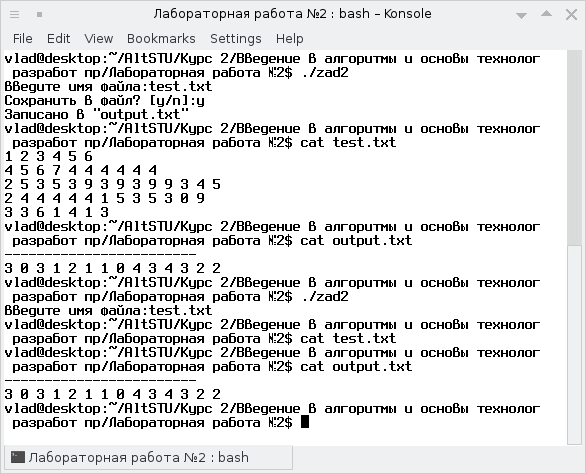
\includegraphics[scale = 1]{1.png}
\end{center}

\end{document}
